\chapter{\label{ch:2-new_conservation_paradigms}New conservation paradigms}
The theoretical and conceptual framework is at the base of the new practices for conserving live media art. As we have seen, universities play a significant role in promoting research initiatives, and it is precisely from the interaction between universities and museums that much of the humanistic and philosophical literature emerges. This literature provides the foundation, perspectives, and future directions for conservation practices. Examples include books published by universities or institutions (e.g., ZKM), journals and special issues dedicated to this field, conferences, doctoral theses, and university courses (as briefly discussed in the previous chapter) that generate and disseminate textual material. This body of literature has contributed to redefining essential elements of conservation, such as the term “conservation” itself, as well as concepts like the authenticity and identity of artworks, which have already been debated in the context of various initiatives.\\
In this chapter, we will explore this theoretical and conceptual framework to deepen our understanding of the ideas underpinning the initiatives analysed in the previous chapter. We will especially examine the latest developments in this field. The main goal is to identify and define the new paradigms for conserving live media art through a synthesis of the intense speculative process occurring in this area of research. These paradigms will form the basis for the model presented in the next chapter.\\
We will begin by examining the role of documentation in conservation and, more broadly, in museums and exhibitions. This analysis will serve as a starting point for exploring the relationship and interaction between the concepts of authenticity and identity. From there, we will propose a new definition of conservation for live media art, focusing on the process that determines it—a loop between documentation and reactivation. Reactivation, another key term in this text, will be discussed in detail. At the end of the chapter, based on the paradigms analysed, we will define the comparison of the live media artwork with a living organism that, through conservation, survives and adapts in an ever-changing exhibition ecosystem.  

%%%%%%%%%%%%%%%%%%%%%%%%%%%%%%%%%%%%%%%%%%%%%%
%%%%%%%%%%%%%%%%%%%%%%%% DOCUMENTATION
%%%%%%%%%%%%%%%%%%%%%%%%%%%%%%%%%%%%%%%%%%%%%%
\section{The role of documentation}
Contemporary museums cease to be places of contemplation and meditation and drop the promise of materialistic eternity. We need to rethink the way we see, handle and study art. We should start talking about \textit{art rheology}, as Borys Groys proposes in his book \textit{In the Flow }\cite{groys2016flow}. The concept of rheology extends from the creation and presentation to the collection, conservation and reactivation of the work of art. Defined and fixed art objects have disappeared from the museum, which now presents events, performances, and installations with a dynamic and transient nature. The ``material'' here is the spatio-temporal context activated by biological, natural and artificial processes.\\
Consequently, conservation—aimed at maintaining an ``original'' state—must also consider dynamicity. When the artwork (the event, performance, or installation) is deactivated, what remains? What must be collected, conserved, and passed on to the future?\\
Live media art in new museums can only last through documentation, much like in theatres and concert halls. Often, documentation is the only thing left after the artwork is no longer active \cite{depocas2002digital}. 
\begin{quote}
“[…] in visiting contemporary museum exhibitions, we are confronted with the irreversibility of time […] the only things that remain will be the documentation: a catalogue, or a film, or a Website” \cite{groys2016flow}.
\end{quote}
While the artwork may have some physical parts, its primary value shifts to the spatio-temporal experience activated. This experience can not be treated and conserved like traditional art but can be documented. Because of this, in museums, as well as in creative and conservation processes, there is a significant shift where the focus moves from the artwork to art documentation \cite{groys2008art}. By quoting Groys again: 
\begin{quote}
“Traditional art produced art objects. Contemporary art produces information about art events” \cite{groys2016flow}.     
\end{quote}
Documentation can be found anywhere in the artwork's life cycle. It has several functions and typologies and involves many people with different roles.\\ 
Multimedia documentation is a fundamental component of information: photos, audiovisual recordings, and many other formats of multimedia documentation allow access to the original form of the artwork, how it was displayed and how the public interacted with it. In addition, as one of the main parts discussed in the previous chapter, oral history is often mentioned as a fundamental source of the artwork description. This type of documentation is closely linked to the multimedia one, bringing together the testimonies of the diversity of the individuals who experienced it. In addition to the ``sanctions'' \cite{irvin2005artist} and ``intentions'' of the creator(s) \cite{lichtin2016you}, it also includes statements of people who contemplated or participated in the artistic event. An example is the audience’s oral history \cite{costello2005understanding, muller2008experience, muller2008towards, jones2008david} already presented in the previous chapter.\\ 
All these documentation elements are essential for returning high-level information about the artwork and describing the behaviour of some kind of organism in relation to time, space and other living organisms. Still, they do not provide (or only partially) information about its constitution and the rules that govern it. In this perspective, we must provide technical documentation about various artwork components and their relationships and functions. In other words, it includes information about required ingredients and how they should be used to bring living organisms to life. Because of the complexity of artworks and especially their ephemeral nature, as early as the 1990s the analogy with the music score is being used to describe the documentation inherent in the technical and realisation aspects \cite{viola1999permanent, van1999between, laurenson2004management, laurenson2006authenticity, rinehart2007media, macdonald2009scoring, noel2011scripting, caianiello2013materializing, rinehart2014re, van2015documenting, phillips2015reporting}.
\begin{quote}
    “When working with media in the context of art, parallels to music are inevitable. Exhibition becomes like a performance or re-creation, an enactment. Active components must be assembled into a complex system to function together according to the artist’s intentions. In the absence of the artist/creator, a person with previous training or experience with the piece and/or a “score,” or set of instructions, is required” \cite{viola1999permanent}.
\end{quote}
If we encounter documentation at various points in the artwork’s life cycle, we must also consider its different roles and purposes at specific moments (as we have also discussed in the previous chapter, concerning the DOCAM project). Figure~\ref{fig:c2-documentation} summarises the different documentation functions in various stages of the artwork.
\begin{figure}[!h]
    \centering
    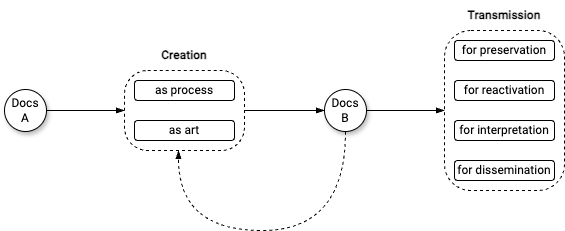
\includegraphics[width=\linewidth]{chapters/2-new_conservation_paradigms/image/graph02-documentation.png}
    \caption{Documentation functions in different stages of the artwork life cycle.}
    \label{fig:c2-documentation}
\end{figure}
Considering the figure, a first distinction has to be made between the \textit{documentation used in the artwork} (\textit{Docs A}) and the \textit{documentation produced from the artwork} (\textit{Docs B}).\\
The first type of documentation (\textit{Docs A}) refers to documents used in the creative process of the artwork. Documentation can be used as a tool for making decisions about the nature and the development of the artwork (documentation \textit{as process}) \cite{dekker2018collecting}. A practical example of documentation \textit{as process} is the work carried out by the media artists group Blast Theory, which used a series of questionnaires, interviews and exercises aimed at the group members themselves and people outside the project to guide the development of the game \textit{Uncle Roy} \footnote{More details about the art project can be found in the Blast Theory website at the link \url{https://www.blasttheory.co.uk/projects/uncle-roy-all-around-you/} (last accessed: 20/09/2024).}\cite{dekker2018collecting}. Documentation can also function as art itself (documentation \textit{as art}). Documentation can refer to a photo, a video, a painting, and other media used to document something and presented in art spaces and through different art forms (e.g. installation). 
\begin{quote}
    Documentation as art means “to use artistic media within art spaces to refer to life itself, that is, to pure activity, to pure practice, to an artistic life, as it were, without presenting it directly.” \cite{groys2008art}. 
\end{quote}
The \textit{Life Sharing} project (2002-2003) of the media art duo 0100101110101101.org is a practical example of documentation \textit{as art}. For three years (from 2000 to 2003), the art group made all of their computer content, such as files, emails and account statements, fully accessible to the public, who could read, download and copy it in real time\footnote{More detail about the art project can be found in the website Net Art Anthology at the link \url{https://anthology.rhizome.org/life-sharing} (last accessed: 20/09/2024).}.\\
The second type of documentation (\textit{Docs B}) refers to documents created during the life cycle of the artwork, whose function extends beyond the deactivation and serves for the interpretation, conservation, reactivation and dissemination and, in general, for the transmission of the artwork toward the future. \textit{Docs B} refer to what is left from the artwork, similar to the performance’s residual objects, which are ``\textit{created in the course of making the performance and during repeated performances}'' \cite{holling2016aesthetics} and once the performance ends, they are the only things left behind, holding memories that can unfold in the present \cite{brignone2009so}. Since the ephemeral nature of live media art, this documentation is the only material that allows for studying, interpreting and reinterpreting an artwork (documentation \textit{for interpretation}). Documentation reflects the understanding of artworks and artistic activities in relation to current and past social and aesthetic values and significance \cite{heydenreich2011documentation:ch7}. It allows for capturing a range of parameters that define the artworks as such, which are crucial for conserving them for posterity \cite{giannachi2022use}. Indeed, documentation is fundamental for conserving the artwork (documentation \textit{for preservation}). 
\begin{quote}
“Documentation provides a tool for monitoring, assisting conservation management and guiding the process of conservation and restoration treatments” \cite{heydenreich2011documentation:ch7}.     
\end{quote}
By interpreting the artwork, we gain insight into what needs to be conserved and the best methods to preserve it, assessing potential risks and ideal conditions \cite{heydenreich2011documentation:ch7}. Consequently, by conserving the artwork, we gain information on how to reactivate it (documentation \textit{for reactivation}). Since it is deactivated, the conservation must consider a new reactivation. Conservation and reactivation can happen through different strategies (like emulation, migration, and virtualisation), but the right approach can only be chosen based on proper documentation. Documentation is generally a tool for communicating and informing about ephemeral artworks across current and future audiences (documentation \textit{for dissemination}).\\ 
However, the documentation that comes from the artwork (\textit{Docs B}) should be understood as something other than merely records or remnants, with only the aim of conserving and presenting the past. Indeed, such documentation should be considered future-oriented \cite{dekker2022documentation, giannachi2022use}. The documentation is not only a derivative of the artwork but also a source for reinterpreting the same work or creating new ones. 
\begin{quote}
“In this sense documentation not only future-proofs but also relentlessly (re-)invents and so (re-)becomes the artwork” \cite{dekker2022documentation}.     
\end{quote}
The installation \textit{Quadrille} by Rose English at Tate is a clear example of an artwork transformed through its documentation over time. The current installation represents the latest stage in the artwork’s evolution. Initially exhibited as an installation in 1974, it was later reimagined as a performance in 1975, incorporating elements from the 1974 installation. Today, it returned to being an installation, this time incorporating costumes, photographs, and videos from the 1975 performance\footnote{Further information about the artwork cna be found in \url{https://www.tate.org.uk/life-artwork-quadrille-rose-english} (last accessed, 4/12/2024)}. Another example is \textit{Il tempo consuma} (1978) by Michele Sambin (a case study carried out by this thesis project\footnote{Please refer to the Appendix~\ref{ax:a-michele_sambin_videoloop} for further information about the case study.}), in which the artist reuses the audiovisual documentation of the first performance inside the digital-reactivated performance or reinterprets the interactive video performance as a static video installation. However, documentation can also serve as a source for creating new artwork. Some examples are the \textit{Reenactments} (2007-2010) of historical performances made by the already mentioned art duo 0100101110101101.org. Instead of simply re-showing and presenting the documentation produced by the original performances (photos and videos), they recreated and performed them inside the video game Second Life, creating a series of new artworks. The duo performed live \textit{Reenactments}, recorded them, and installed them in different formats\footnote{ The performances reenacted are \textit{Seedbed} by Vito Acconci, \textit{Imponderabilia} by Marina Abramovic and Ulay, \textit{The Singing Sculpture} by Gilbert \& George, \textit{Shoot} by Chris Burden, and \textit{Tapp und Tastkino} by Valie Export and Peter Weibel. Some of the video recorded can be found in the duo’s website at the link \url{https://0100101110101101.org/reenactments/} (last accessed: 20/09/2024).}.\\
The live media art documentation process is an accumulation of information, or, as named by Hanna Hölling, a \textit{stratigraphy of documentation} that ``\textit{may never cease to expand, continually depositing new layers on the already accumulated sediment}'' \cite{holling2016aesthetics}. Therefore, in a later article Hanna Höllings proposes to see the work as an archive that is not only a repository of documents but also an ``\textit{intangible, non-physical realm of tacit knowledge and memory in an ever-enduring state of organisation and expansion,}" \cite{holling2017paik} a dynamic entity from which the artworks are actualised and to which they contribute \cite{van2024conservation}.

%%%%%%%%%%%%%%%%%%%%%%%%%%%%%%%%%%%%%%%%%%%%%%
%%%%%%%%%%%%%%%%%%%%%%%% AUTHENTICITY IDENTITY
%%%%%%%%%%%%%%%%%%%%%%%%%%%%%%%%%%%%%%%%%%%%%%
\section{From fixed authenticity to forming identities}
The ephemeral nature of live art and the dynamicity with which documentation is created, accumulated, and used according to artworks raise many questions about authenticity. Questions, discussions, and debates around this concept are born and continue to rise in conjunction with the growing conservation and restoration practices and the establishment of new artistic forms. As briefly mentioned in the previous chapter, live media art proposes a new perspective from which to define authenticity compared with traditional art forms. For this reason, the speculative process around this artistic field has been and continues to be highly heated.\\
In the conservation and restoration context, the concept of authenticity began to be established in the 19th century, especially after the second-post world. The term was bound to the preservation of physical and material aspects of an artwork. Among the most important texts to affirm such an idea are the \textit{Theory of Restoration} (1963) by Cesare Brandi \cite{Brandi2005theory} and the \textit{International Charter for the Conservation and Restoration of Monuments and Sites} (1964) \cite{venicecharter1964} drafted by UNESCO’s \textit{Second Interaction Congress of Architects and Technicians of Historic Monuments}. Both texts refer to the authenticity of art forms such as sculpture, architecture and painting. These artworks are considered to have original ``state'' or ``condition,'' which are identified and revealed in the material and physical evidence. The material and physical evidence can be authenticated, i.e., allowing the identity of an artwork to be defined as a product derived from a human creative process belonging to an author to whom it has been attributed. Therefore, authenticity is used to identify the artwork’s truthiness, ``\textit{and it is often contrasted with the concept of false or fake}'' \cite{jokilehto2010conservation}.
\begin{quote}
    “On the other hand, taking the contrary, i.e. something inauthentic or fake, this can be defined as an artefact where the sources of information have been altered or falsified” \cite{jokilehto2010conservation}.
\end{quote}
The restoration aims to reveal a work of art’s truthfulness; the conservation aims to maintain its integrity. 
\begin{quote}
    “For the majority of traditional art objects, minimising change to the physical work means minimising loss, where loss is understood as compromising the (physical) integrity of a unique object” \cite{laurenson2006authenticity}.
\end{quote}
Another important text was \textit{The Nara Document on Authenticity} (1994) \cite{naradocument1994}, drafted during a World Cultural Heritage conference in Japan in 1994. In this text, the connection between authenticity and materiality began to unbuckle since the concept of intangible heritage was introduced in the speculative process.\\
Summarising this text and the previous important ones, Jukka Jokilehto generally lists three essential parameters with which to define authenticity up to that time \cite{jokilehto2010conservation}:
\begin{itemize}
    \item \textit{Qualitative judgement} about a work is considered a result of the human creative process and, therefore, autonomous and not a copy;
    \item \textit{Legal verification} about the material truth of an object as a historic document;
    \item \textit{Social-cultural traditions} and inculcation of value judgements.
\end{itemize}
These parameters, especially the link between authenticity and materiality, are wholly blurred in the context of live media art. This art form needs new and specific parameters to consider authenticity and thus conserve the artwork.\\
\begin{quote}
    “If the ontological framework is focused on the material so will the notion of authenticity. If the ontological framework shifts, then we expect a similar shift in our concepts of authenticity, change and loss” \cite{laurenson2006authenticity}.
\end{quote}
In his writings, Pip Laurenson \cite{laurenson2004management, laurenson2006authenticity} introduces two essential philosophical concepts that underpin the speculative debate on the authenticity of live media art. These concepts are the \textit{autographic-allographic distinction} defined in \cite{goodman1968languages} and the \textit{two-stage model} in \cite{davies2001musical}.\\
In Language of Art \cite{goodman1968languages}, Nelson Goodman introduces the \textit{autographic} and \textit{allographic} terms within the authenticity context, aiming to separate two scenarios in artistic creation: the forgeable and non-forgeable arts, the arts such as sculpture and paintings and arts such as music and theatre.
\begin{quote}
    “Let us speak of a work of art as autographic if and only if the distinction between original and forgery of it is significant; or better, if and only if even the most exact duplication of it does not thereby count as genuine. If a work of art is autographic, we may also call that art autographic. Thus painting is autographic, music non-autographic, or allographic. [...] One notable difference between painting and music is that the composer’s work is done when he has written the score, even though the performances are the end-products, while the painter has to finish the picture. No matter how many studies or revisions are made in either case, painting is in this sense a one-stage and music a two-stage art.” \cite{goodman1968languages}
\end{quote}
Autographic refers to art where the physical, original object matters. If one attempts to create an exact duplicate of the work, it would be considered a forgery, not an original. Its opposite, the allographic, is an art where the work’s identity is not tied to any particular physical object but rather to a set of instructions or a notation system. Copies or reproductions of these works can still be considered authentic as long as they follow the original notation or instructions.
\begin{quote}
    “In sum, an established art becomes allographic only when the classification of objects or events into works is legitimately projected from an antecedent classification and is fully defined, independently of history of production, in terms of a notational system. Both authority and means are required; a suitable antecedent classification provides the one, a suitable notational system the other. Without the means, the authority is unexercised; without the authority, the means are footless.” \cite{goodman1968languages}
\end{quote}
In \textit{Musical Works and Performances: A Philosophical Exploration} \cite{davies2001musical}, Stephen Davies, following the Goodmanian distinction, introduces the \textit{two-stage model}. The model consists of a composition stage (the first stage) in which the music composition is created and written down through a notational system (i.e. through the compilation of the score) and a performance stage (the second stage) through which the musical work is realised. Each performance is a unique interpretation, providing different perspectives of the original work. The resulting interpretation could be more or less aligned with the original composer’s intention, but it is still rooted in the compositional framework established in the first stage. This model acknowledges that while a score represents the idealised work, each performance contributes to the work’s identity.\\
Pip Laurenson places live media art ``\textit{on the ontological continuum somewhere between performance and sculpture},'' defining it as allographic since it is ``\textit{similar to works that are performed}'' and therefore belongs to those artworks ``\textit{created in a two-stage process}'' \cite{laurenson2006authenticity}. In this context, as required by both the allographic concept and the \textit{two-stage model}, live media art demands a score, better described as \textit{work-defined properties}, usually provided by the artist.\\
\textit{Score compliance} (Castriota, 2024) is essential for defining authenticity in live media art. In this context, the ``score’’ is not an entirely accurate analogy because, due to the diversity of art and related terminological issues, creating a general notation system is unattainable. The score in live media art refers to all the residual documentation (previously called \textit{Docs B}), which helps establish the artwork's \textit{textual stabilisation} \cite{holling2016aesthetics} or, as already mentioned, all the \textit{work-defined properties} in written form. These aren’t just scores (borrowed from the musical context to describe the graphic representation of performance events in space and time) but also instructions, scripts, testimonies, etc. In the absence of the original object, the documentation defines and builds the artwork's identity. Documentation is essential to guide new versions of the artwork, which would be more or less authentic.\\
So, while in autographic art, the parameters of change and loss are discussed according to material and physical authenticity, in allographic art, the idea used to consider the parameters of acceptable change is identity \cite{laurenson2006authenticity}.\\
Moreover, while in traditional conservation, we consider authenticity based on the original state of an object's creation, in live media art, as highlighted by the new documentation's role previously discussed (and shown in Figure 1), we cannot define a fixed but rather \textit{variable} \cite{groys2008art}, or better yet, \textit{under construction} \cite{dekker2022documentation} or \textit{forming} (Phillips, 2015) identity.
\begin{quote}
    "it was recommended that changes in an artwork should be tracked by iterative documentation. In recognising that artworks change, the use of the term ‘original’ started to be avoided, in that it had become clear that it is often impossible to tell which version of an artwork may be the ‘original’ or whether one could even still talk of originals, suggesting, perhaps, that there may not be any difference between various versions of a work". \cite{giannachi2022use}
\end{quote}
Joanna Phillips’ \textit{Documentation Model for Time-Based Media Art} illustrates the idea of forming identity, which establishes a clear distinction between the artwork’s score and its manifestations. All the elements (documentation) that define the work's identity are grouped within the score, while the manifestations represent various interpretations of that score. Although this model resembles Davies’ \textit{two-stage} model, it is an extension. Phillips emphasises that when an artwork enters a collection (or after its first manifestation), it enters a ``state of infancy,'' and its various manifestations contribute to the process of ``forming its identity'' \cite{phillips2012shifting, phillips2015reporting}. This perspective shifts the relationship between identity and authenticity from a unidirectional one to a more bidirectional dynamic.\\
The idea of fixed, original authenticity is replaced by an identity shaped through the different versions or manifestations of the artwork. In Figure~\ref{fig:c2-authenticity}, we summarise the relationship between concepts of authenticity and identity in various art forms. In autographic art, the identity is inscribed inside the authenticity, which can be found in the artwork's original state, which can be restored and preserved. The allographic art’s identity is fixed in a score and informed through different performances of such a score, which can be more or less authentic. Here, we can introduce the concept of dynamic authenticity introduced by Perla Innocenti \cite{innocenti2012bridging, innocenti2012rethinking} to describe the authenticity of performances and non-physical art. Live media art, while often categorised as allographic, surpasses this definition. The artwork's identity evolves as documentation accumulates—encompassing a wide range of materials beyond just a musical score. Therefore, live media art combines the concept of dynamic authenticity with the notion of an identity that is continually forming. Pip Laurenson refers to live media art with the idea of ``epistemic objects'', i.e. objects that are open, incomplete, and whose significances continually emerge through their indefinite ``unfolding'' \cite{laurenson2016practices}. Castriota extends the concept of forming identities by questioning the concept of \textit{centring} in the identity construction of an artwork\footnote{Introduced by Castriota in \cite{castriota2018centres} as the process of drawing hard lines around an artwork’s essential properties.}, introducing the idea of a \textit{multiple perspectives identity} and \textit{multiple centres} \cite{castriota2019authenticity, castriota2024enfolding}.
\begin{figure}[!h]
    \centering
    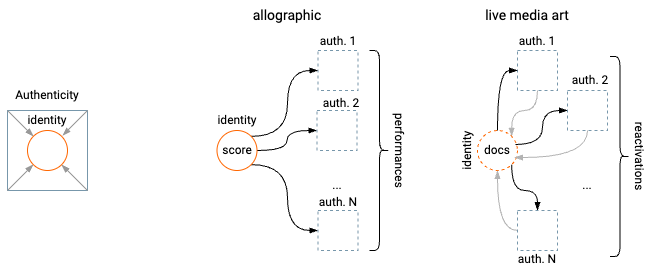
\includegraphics[width=\linewidth]{chapters/2-new_conservation_paradigms/image/graph02-identity.png}
    \caption{Three different models which show the different relation between authenticity and identity in autographic, allographic, and live media art.}
    \label{fig:c2-authenticity}
\end{figure}

\section{The conservation loop}
If the concepts of authenticity and identity change, the activities related to these concepts, such as conservation, preservation, and restoration, also change. Like authenticity, these terms lack an absolute definition. They have been used differently throughout history and across different fields. To resolve this confusion –at least within this text–we will use the definitions of conservation, preservation, and restoration as defined in the context of the essay \textit{Contemporary Theory of Conservation} by Salvador Muñoz Viñas (2005), often used as a reference in literature \cite{munoz2005contemporary}. The author does not define these activities with the goal of fixing absolute meanings but rather as a reference within his book.\\
Muñoz Viñas uses the term ``conservation'' in a broad sense, as the sum of activities aimed at keeping an artwork as it is, plus activities intended to restore the artwork to an ``original nature'' or ``previous version.'' Therefore, this term is considered to encompass both preservation and restoration activities. Preservation can be defined as an activity intended to keep something as it is, maintaining its integrity and thus avoiding alterations and minimising deterioration, with the goal of extending the life expectancy of cultural heritage. However, in reality, preservation involves an intervention in the object, which means it cannot happen without some alteration. The author notes, ``\textit{[p]reservation could thus be defined as the action intended to keep the perceivable features of an object in the present state for as long as possible – a goal which is usually achieved by modifying some of the object's non-perceivable features}.'' Among the different definitions mentioned in the book, for which the author highlights some inaccuracies, he uses the definition of restoration given by the Museum and Galleries Commission, which defines it as ``\textit{all action taken to modify the existing materials and structure of cultural property to represent a known earlier state}" \cite{mgc1994}. Therefore, in contrast to preservation, the author states that ``\textit{restoration can be defined as the action that attempts to modify an object's perceivable features}'' in order to return the object to an earlier state.\\
Restoration and preservation are activities primarily focused on an artwork's present and past states, particularly when referring to physical objects. In the context of live media art, however, the focus of conservation shifts to the experience. For this reason, strategies like storage, migration, emulation, and re-interpretation are proposed as contemporary preservation methods. Since the object of preservation is the experience created by the artwork, these interventions can be considered non-perceivable and evaluated based on a degree of authenticity, much like in musical performances. Interventions on software and hardware (such as migrations and porting) are considered non-perceivable (depending on the specific artwork) since they are part of an assembly that activates the experience, which is the perceivable element.\\
However, the concept of preservation and restoration makes sense when applied to a physical, material object, but it becomes weak when applied to an experience. The experience of an artwork cannot be preserved; Again, it can only be documented. The experience is not only created by the assembly and activation of hardware and software components but, more importantly, by the viewers. Socio-cultural factors shape a person's experience of a work of art or technology. Therefore, when reactivating a live media artwork, it is difficult to talk about maintaining a specific ``state'' or ``condition,'' whether present or past. Instead, supporting the discussion of authenticity mentioned earlier, each reactivation always generates a new experience.\\
Consider \textit{Hole in Space} by Kit Galloway and Sherrie Rabinowitz, a telecommunication art installation that connected people in real-time between two distant locations—Los Angeles and New York City. In the 1980s, this real-time connection across these two cities, several kilometres apart, created a truly impressive, almost science fiction-like experience, perfectly reflecting the installation’s title. However, in today’s world, where real-time global communication is a daily norm, a direct reactivation of the artwork would not evoke the same impact. Recognising this, in 2023, MoMA chose to reactivate the work using a reinterpretation approach. Instead of replicating the original setup, the reactivation relied on documentation from the 1980s to reimagine the experience\footnote{More details about the artwork can be found in the MoMa website, at the link \url{https://www.moma.org/collection/works/120330} (last accessed 13/12/2024).}.\\
This preservation aspect also arose during a case study conducted during this project thesis, specifically in the reactivation and presentation of \textit{Caos delle Sfere} by Carlo De Pirro\footnote{More details about the case study can be found in Appendix~\ref{ax:b-hybrid_reactivation_il_caos_delle_sfere}.}. \textit{Il caos delle Sfere} is a sound installation from 1999 based on an interactive system involving a pinball machine and a Disklavier, which communicate through a computer with dedicated software. The reactivation raised interesting considerations, mainly due to the presence of the pinball machine. In 1999, when the artwork was first presented, pinball machines were common and could be found in many public spaces. The pinball machine has almost entirely disappeared today, resulting in an entirely different impact. For older people, it is a memory; for younger generations, it is a ``novelty.'' As a result, the focus shifted entirely from the interaction between the game and the music to the pinball machine as a historical device, completely altering the experience of the artwork.\\
Therefore, if we consider the experience of the artwork as the ``object'' of conservation, the conservation process itself needs to be redefined. Whether there is a preservation intervention (like migration or emulation), a re-interpretation, or an extremely faithful restoration, the artwork (or experience) will always change. This change is part of what we discussed earlier—the process of forming and shaping the artwork’s identity.\\
Conservation, whether in traditional, autographic, allographic, or live media art, is always about identifying the artwork or, more accurately, defining its identity. In traditional art, conservation assumes that the identity, tied to the artwork’s authenticity, is either revealed (through restoration) or maintained (through preservation). In live media art, however, conservation involves constructing or shaping the artwork’s identity by keeping the essential elements alive so the work can continue to unfold.
In this context, the concept of ``safeguarding'' (Blutter, 2018; Castriota, 2019) is introduced as the opposite of preservation:
\begin{quote}
    "Preserving seeks to secure the life that already is; safeguarding secures and reproduces the conditions of becoming, of living, of futurity, where the content of that life, that living, can be neither prescribed nor predicted and where self-determination emerges as a possibility." \cite{butler2018my} 
\end{quote}
So, while preservation is an activity aimed at fixing the state of something to pass it on to the future, safeguarding aims to maintain the necessary conditions for something to continue to exist (without necessarily being aware of how it will change in the future) \cite{castriota2019authenticity}. Rebecca Gordon names that ``something'' \textit{critical mass}: ``\textit{the optimum choice and grouping of factors or attributes that demonstrate the core identity of the work of art}'' without which the work could not continue to exist \cite{gordon2014identifying}.
\begin{quote}
"safeguarding aims to simply secure the conditions for its future to remain a possibility, a future wherein its identity may evolve, diverge, or multiply." \cite{castriota2019authenticity}
\end{quote}
Therefore, the new concept of conservation–as the action of safeguarding– can be established in a loop between documentation—everything that remains of the artwork after its deactivation, which ensures its survival—and reactivation, which is the transcription and transmission of the artwork that occurs through various methods, always starting from the documentation. This relation between documentation and reactivation is a loop because each reactivation shapes the artwork’s identity and creates new conditions for survival that need to be documented. Figure~\ref{fig:c3-conservation} summarise the differences between traditional and live media art conservation.
\begin{figure}[!h]
    \centering
    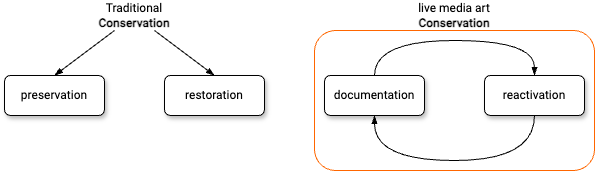
\includegraphics[width=\linewidth]{chapters/2-new_conservation_paradigms/image/graph02-conservation.png}
    \caption{Traditional and live media art conservation paradigms.}
    \label{fig:c3-conservation}
\end{figure}

\section{Reactivation: transcription and transmission}
The term reactivation definitely deserves further exploration, as it is not very common in the literature (though it has been used more frequently in recent years). When used, it is often unclear or confused with terms like \textit{reenactment}, \textit{reconstruction}, \textit{reinterpretation}, and \textit{replication}. As highlighted by Auslander in \textit{Reactivation: Essay on Performances and its Documentation} (2019), the use of this term dates back almost a century \cite{auslander2018reactivations}. It appears in one of the most important contemporary art texts, \textit{The Work of Art in the Age of Mechanical Reproduction} by Walter Benjamin, written in 1935 \cite{benjamin1935work}. In his essay, Auslander introduces Benjamin's concept of reactivation, using Benjamin's own words, such as:
\begin{quote}
    “Technical reproduction can put the copy of the original into situations which would be out of reach for the original itself. Above all, it enables the original to meet the beholder halfway, be it in the form of a photograph or a phonograph record. The cathedral leaves its locale to be received in the studio of a lover of art; the choral production, performed in an auditorium or in the open air, resounds in the drawing room [...] the technique of reproduction detaches the reproduced object from the domain of tradition. By making many reproductions it substitutes a plurality of copies for a unique existence. And in permitting the reproduction to meet the beholder or listener in his own particular situation, it reactivates the object reproduced." \cite{benjamin1935work}
\end{quote}
Benjamin's essay is well-known for its concept of ``aura'' in the context of technical reproduction. The technical reproduction of an artwork deactivates the original, removing it from its historical and local context, thereby stripping it of its authenticity and authority. As a result, technical reproduction takes away the ``aura'' of the original. However, in the excerpt just mentioned, Benjamin also introduces the concept of reactivation, which, as Auslander points out, is often overlooked in the analysis of this famous essay. Technical reproduction does not return the artwork to its original time and space; rather, it places it in a new and current moment and space of experience. Each time the reproduction is ``observed,'' the original artwork is reactivated as a production in the present, not as a replica of a historical past. Therefore, when reactivated through interaction with an observer, reproduction functions as a \textit{post-auretic object} \cite{auslander2018reactivations}.\\
Although slightly different, the writings of Nelson Goodman \cite{goodman1982implementation, goodman1998art} include the terms \textit{activation} and \textit{implementation}, which are very useful for analysing the concept of reactivation in live media art. Both terms refer to all the actions, usually carried out by curatorial projects, that maximise ``\textit{the functioning of the work as a work of art and as that particular work - that is, bringing about insight into and understanding the work}” \cite{goodman1982implementation}. Many activities fall under this umbrella, such as the placement of light, the juxtaposition of two works, the development and placement of a caption, the creation of an exhibition, the publication of a catalogue, and so on. The examples in the essay \textit{Art in Action} (1998) show how these actions are important from the perspective of live media art and in relation to Benjamin's concepts of reproduction and reactivation. The examples include using light to activate paintings, which connects to another example involving the cleaning and care of the artwork ("\textit{cleaning it and lighting it are here partners in activation}"), as well as the conservation of murals and manuscripts, culminating in activation through reproduction.\\
In the context of activation for conservation, Goodman gives a very interesting example: the interventions at the \textit{Lascaux Caves} in southern France. These caves contain 600 ancient murals, estimated to be around 17,000 years old. After being discovered in 1940, the murals began to deteriorate due to exposure to air and humidity caused by the presence of thousands of visitors each day. As a result, the caves were closed in 1963. A full-scale replica of the cave was created in 1980 to activate this archaeological and artistic space and thus enhance access and understanding of the artwork for a wider audience.\\
Another example of activation, which aligns with Benjamin's concept of reactivation, is reproduction, including ``\textit{photographs, transparencies, slides, illustrations in books, and so on.}`` These are not merely ``\textit{replacements, substitutes, surrogates, or proxies for the original}'' but rather tools through which we can activate a work: ``\textit{laypeople and experts alike know or understand most works of art through reproductions}." Goodman refers to this type of activation as indirect activation, where "{action at a distance, or even posthumous action, is possible}'' \cite{goodman1998art}.\\
In essence, Benjamin views reactivation as the interaction between an observer and the reproduction of a work of art. Using the terms \textit{activation} and \textit{implementation}, Goodman refers to the actions taken (usually by experts, curators, or conservators) that enable access to the artwork, thus allowing interaction with an audience.\\
In the context of live media art, specifically for this text, we want to define reactivation to include both meanings. Reactivation encompasses actions aimed at presenting the deactivated artwork in a new space-time context and its resulting interaction (or observation) by a new audience. Therefore, we can define reactivation as the sum of \textit{transcription} and \textit{transmission}\footnote{Terms already presented in the previous chapter in the context of preservation strategies. Transmission, reinscribing and transmission were proposed by the \textit{Archiv Performativ} project.}. By \textit{transcription}, we mean all actions aimed at providing new access to the deactivated artwork, ranging from ``\textit{historical faithfulness to the ‘original’ in reenactment, through interpretative translation in re-performance, to reformulation or transformation in an artistic work}''. Therefore, the \textit{transcription} can be accomplished through different preservation strategies (storage, emulation, migration, reinterpretation, virtualisation, etc.) and \textit{reinscribe} specific artwork aspects. \textit{Transmission} takes place once the artwork has been implemented and thus meets and interacts with the observer, creating a new experience in the new space-time context.

\section{The ecological turn}
At this point, we should ask ourselves how, through all these reactivations, new transcriptions, and transformations—both in the artwork’s presence and in the resulting experience—we can still perceive the artwork as the same specific artwork. How can we track its identity? We might wonder whether the artwork is still the artist’s work or an interpretation by the conservator. Is it then an interpretation of an interpretation? In its unfolding, its formation, and the decentering of its identity, how does that specific work remain the same?\\
Regarding the traceability of the artwork’s variability, Van De Vall and Hollings introduce the concept of \textit{cultural bibliography} in conservation practices \cite{van2011reflections}. Once the artwork enters the museum or the conservator’s hands, it does not stop or die but continues to grow and evolve, developing its biography.
\begin{quote}
“The central idea of the biographical approach is that the meaning of an object and the effects it has on people and events may change during its existence, due to changes in its physical state, use, and social, cultural and historical context” \cite{van2011reflections}.  
\end{quote}
With this approach, the metaphor of the artwork as a living being can be introduced. A living being with its own history, which we can trace through its biography. Similarly, Van Saaze uses the term \textit{career} to describe the variability of the artwork (as defined also in \cite{becker2006art}) and proposes viewing it through \textit{actor-network theory} (ANT) \cite{van2013installation}. According to ANT, the artwork, like other human and non-human entities, is an \textit{actant}—an entity capable of acting or influencing (and, of course, being influenced by) other entities within a network. Thus, through ANT, the artwork is not given once and for all; instead, it occurs repeatedly as a result of the conservation practice itself. The goal of conservation is to find and analyse the transformations of the actants that have shaped the artwork and to reintroduce them into renewed interactions within a network to continue defining the artwork as that specific piece.\\
We define the network of entities interacting to determine the artwork as the \textit{exhibition ecosystem}, which we define here as a second-level ecosystem. The entities (or actants) that interact with and determine the artwork are drawn from other ecosystems, which we refer to as first-level ecosystems. Here, we identify three main first-level ecosystems: the \textit{media and technology ecosystem}, the \textit{institutional ecosystem}, and the \textit{authorship ecosystem}\footnote{These ecosystems are derived from the definition provided in \cite{rinehart2014re} of three external threats that can endanger the future of a live media artwork: \textit{death by technology}, \textit{death by institution}, and \textit{death by law} (the latter expanded here as the \textit{authorship ecosystem}). As threats, these represent ecosystems with which the artwork must interact.}.\\
The \textit{media and technology ecosystem} includes both human and non-human entities, such as the technologies themselves (devices, software, etc.), the companies and individuals who work with and develop them, and the people who use them. It is one of the primary ecosystems that raises the most significant challenges in the conservation of artworks, as it forms the basis of most works and is characterised by a rapidly accelerating process of becoming. As we saw in the previous chapter, the issue of obsolescence is a central concern for many conservation initiatives. This problem triggers a chain reaction within the network of people with the knowledge and expertise to work with specific technologies \cite{laurenson2013emerging}. It continuously renews the user experience and quickly turns technologies from just a few years ago into antiquate tools (as seen with \textit{Hole in Space} and \textit{Il caos delle sfere}).\\
The \textit{institutional ecosystem} is also defined by human and non-human entities, including the people who manage and work in the institution, the institution’s space, its archive, and its collection (including the artworks). This ecosystem refers to the institutions responsible for collecting and exhibiting the artwork, typically represented by museums but also by other institutions discussed in previous chapters. Each institution has its own approach to collecting, conserving, and displaying artworks. It brings a network of different institutions and individuals to satisfy, as well as other artworks with which the artwork must communicate.
\begin{quote}
“The artwork is entangled with the museum’s repertoire, organizational structures, work division, politics, documentation procedures, and level of engagement” \cite{van2013installation}.    
\end{quote}
Next, we have the \textit{authorship ecosystem}, which mostly comprises human entities and includes a more or less distributed group of people (distributed authorship) with different roles. This ecosystem not only plays a creative role but also provides support, including legal guidance on access and usage rights for the artwork or its components.\\
In addition to these omnipresent ecosystems—though they have different balances in each case—there could be other specific entities from other first-level ecosystems that come into play, depending on the artwork. For example, site-specific works engage a unique \textit{space ecosystem} that becomes essential for their realisation.\\
Entities in interaction within and between these ecosystems are put into further interaction within the second-level \textit{exhibition ecosystem}, where the artwork itself becomes an actant. The \textit{exhibition ecosystem} is created through negotiation between the first-level ecosystems so they can interact in relation to the artwork. This negotiation is made possible and limited by the artwork’s \textit{changeability}, which is both its potential to change \cite{holling2017paik} and the limit beyond which an artwork ceases to be the same \cite{van2023theories}. This negotiation defines the artwork’s transformation or variability. The new conservation paradigms establish the basis for this negotiation so that the transforming and growing artwork can no longer be viewed as a fixed entity but rather as an organism adapting to the transformation of an indirect (second-level) ecosystem, made possible by continuous negotiation.\\
To answer the question posed at the beginning of this section, we propose using what Van De Vall refers to as the \textit{ecological turn} in conservation thinking \cite{van2023theories}. According to this approach, the transformation of the artwork, its development and formation over time, should be understood within the context of its environment—its ecology of interactions between the various entities that define the conditions for the artwork’s existence, persistence, and becoming. The \textit{biography} and \textit{career} of the artwork, as well as its forming identity, cannot be defined except as the result of conservation practices, which determine the artwork’s ecology. Therefore, as Van De Vall asserts, in radical cases, it is the very ecologies that produce the ontologies of the artwork:
\begin{quote}
“Rather than deriving conservation practices from the works’ ontology, these ontologies are considered to be the results of these practices.” \cite{van2023theories}    
\end{quote}

\section{Summary}
In this chapter, we defined the fundamental paradigms of live media art conservation. We explored how the artwork becomes a living organism, an \textit{actant} that interacts with and transforms within the \textit{exhibition ecosystem}—a network of complex, constantly changing entities. The artwork is defined within this network, without which it cannot exist. Therefore, conservation practices here are understood as actions aimed at keeping the artwork alive—negotiating with the involved entities and continuously building the interactions that define the artwork. Conservation, then, is no longer about discovering the artwork’s identity but about constructing it, surpassing both the concepts of \textit{autographic} and \textit{allographic} works. This identity is in formation; it develops, grows, matures, and eventually ages and dies. As we’ve seen, this process happens through a potentially endless loop between \textit{documentation} and \textit{reactivation}. Documentation plays a central role in conservation, taking many forms and serving multiple purposes in relation to the artwork and its life. Only with proper documentation we can consider the reactivation of artworks that cannot be physically conserved. Reactivation is the process by which the artwork is \textit{transcribed} through a new balance of interactions between the involved entities, meaning the work is reconstructed from the \textit{documentation} and transmitted through the exhibition ecosystem to these entities, generating a new spatio-temporal experience and creating a new chapter in the artwork’s \textit{biography}.\\
In other words, the past is no longer the goal of conservation. Instead, the past is a tool that conservators use to create the conditions under which the artwork can continue to exist in the present and future. Therefore, the artwork in its current state is no longer the exclusive result of a single artist but rather a collective contribution formed throughout its lifespan, from its creation through its conservation.